
%----------------------------------------------------------------------------------------------------------------------------------------

% définit le type de document et ses options
\documentclass[a4paper,10pt]{article}

% des paquetages indispensables, qui ajoutent des fonctionnalites
\usepackage[utf8]{inputenc}
\usepackage{graphicx}
\usepackage{lscape}
\usepackage{url}
\usepackage{xspace}
\usepackage[francais]{babel}
%\usepackage{fullpage}

\pagestyle{plain}


%----------------------------------------------------------------------------------------------------------------------------------------


% le debut du contenu
\begin{document}


%----------------------------------------------------------------------------------------------------------------------------------------


%%%%%%%%%%%%%%%%%%%%%%%%%%%%%%%%%%%%%%%%%%%%%%%%%
%%Page d'accueil
\begin{center}
	%%
	\hspace{8cm}
	
\includegraphics[scale=0.8]{logo.ps}

	%%
	\vspace{3cm}
	{\huge Projet de spécialité 2010}\\
	{\huge Conception d'un modèle de feu 3D temps réel}\\
	{\large Compte Rendu de Suivis}\\
	\vspace{1cm}


	\includegraphics[scale=0.3]{feu.ps}\\
	\vspace{2cm}
	%%
	Etudiants impliqués :\\
	Benjamin Aupetit - IRVM - benjamin.aupetit@ensimag.imag.fr\\
	Julien Champeau - IRVM - julien.champeau@ensimag.imag.fr\\
	Arnaud Emilien - IRVM - arnaud.emilien@ensimag.imag.fr\\
	~\\
	Encadrants :\\
	Marie-Paule Cani  -  Marie-Paule.Cani@inrialpes.fr 
	Aurélie Catel - aurelie.catel@grenoble-inp.fr
	~ \\
	\vspace{3mm}
	Ensimag 2010\\

\end{center}

\newpage







%----------------------------------------------------------------------------------------------------------------------------------------
%%%%%%%%%%%%%%%%%
\section{Suivis du  20 mai 2010}
%%%%%%%%%%%%%%%%%
\subsection{Présents}
\textbf{Tuteur} : Marie Paule Cani \\
\textbf{Élèves} : Benjamin, Julien, Arnaud \\
\subsection{Sujet abordé}
\textbf{Définition du but et de l'échelle du projet} :  \\
se concentrer sur la propagation et la destruction des objets.\\
\textbf{Pistes à regarder} : \\
Jos Stam a fait de nombreux travaux à ce sujet, il faut regarder sur son site web de toronto. Par exemple : burning cross. Il a travaillé sur la représentation et  les modèles de feu temps réel.\\
Mathieu Desbrun à fait "Voxels On fire" et "Meshes On Fire", deux travaux sur la propagation temps réel du feu sur un objet.\\
Représentation du feu par voxels.


\textbf{Conseil sur la démarche} : \\
Reflechir beaucoup au BUT,
identifier les phénomènes importants,
lire beaucoup,
faire des résumés régulièrement.

\subsection{Prochain rendez vous}
Lundi 31, à 10h à l'INRIA.\\
Nous devrons y présenter le modèle de feu et de fumée.
%----------------------------------------------------------------------------------------------------------------------------------------
\end{document}
